\documentclass[12pt]{article}

\usepackage{graphicx}
\usepackage[skip=2pt,font=scriptsize]{caption}

\title{Are consecutive annual mean temperatures in a given location
significantly correlated?}

\author{Ben Nouhan, bjn20@ic.ac.uk}

\date{\today}


\begin{document}
\maketitle

\vspace{2mm} 

\setcounter{section}{3}
\section{Results}


We used mean annual temperatures from 100 years, 1901-2000, in Key West,
Florida. The mean of the mean temperatures across all years was  25.31, with a
range of 23.75-36.35 and SD of 0.50 (Fig. 1a). There is a clear positive
correlation between year and mean annual temperature.

When mean temperature of one year is plotted against 
the mean temperature of the next, any correlation that may exist is less clear 
(Fig. 1b). The aim of this study was to determine if there was a such a
correlation, and if so was it statistically significant. Therefore, the null 
hypothesis is that the correlation coefficient is not significantly more than 0, 
and the alternate hypothesis is that it is.

We wanted to test this hypothesis at the 5%
significance level, but unfortunately the lab's statistical tables book set on 
fire in a horrific accident, and the WiFi was down. Hence, we needed to estimate 
the p-value from first principles.

Having calculated the Pearson's auto-
correlation coefficient (ACC) of the data in Fig. 1b, 0.326, this required us to 
randomise the data by 'shuffling' the measured temperatures associated with each 
year, find the autocorrelation coefficient of that randomised data, repeat the 
process 10,000 times, and compare the 10,000 ACCs with the ACC of the real data. 

In order to ensure reproducibility, the seed was set to 294 prior to the 
random sampling. This lead to the distribution of 10,000 ACC values shown in 
Fig. 2.

\begin{figure}[tp!]
\centering
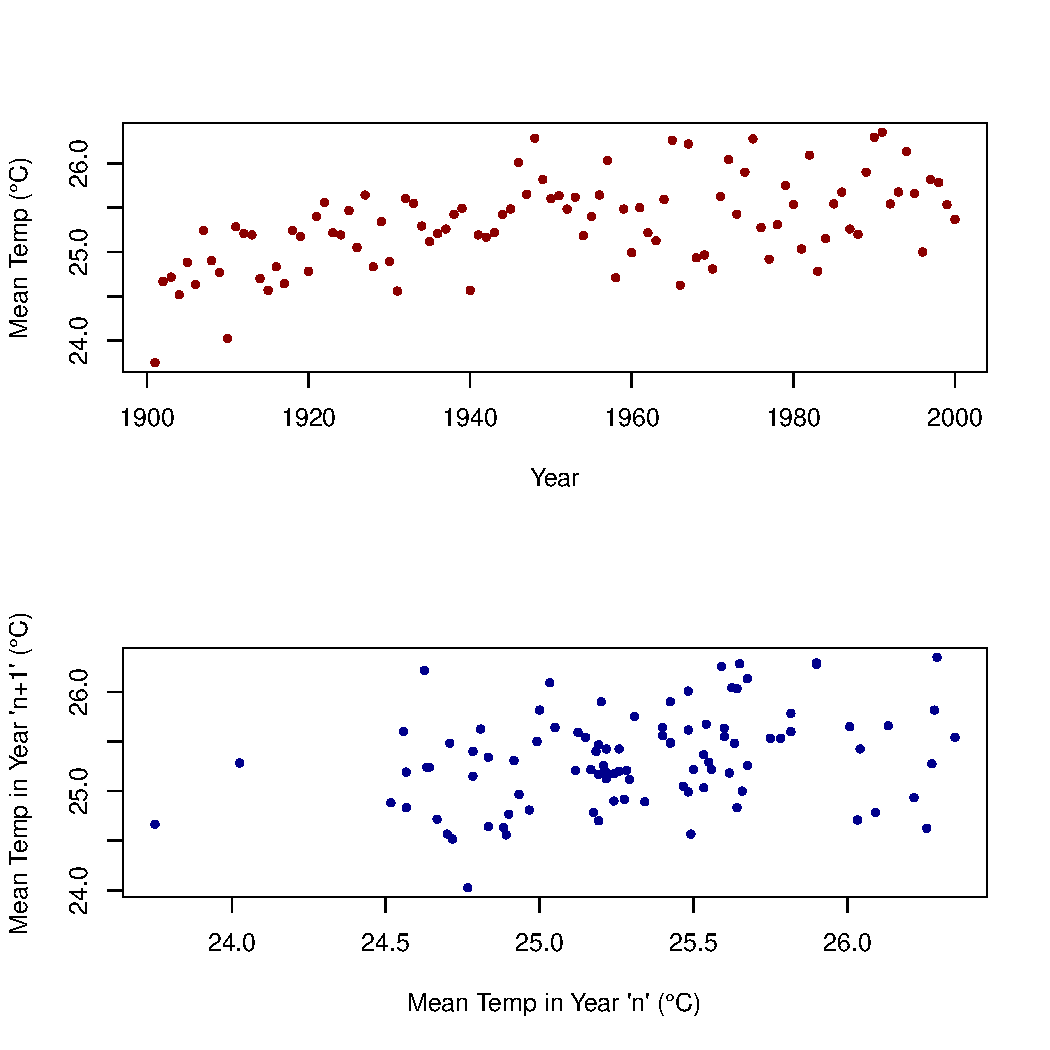
\includegraphics[width = 6in, height = 7in]{../data/ACC_Data.pdf}
\caption{Scatterplots plotting mean annual Temperature against the year it 
was measured (a, above), and the mean temperature of one year against 
the mean temperature of the next (b, below). All temperatures were measured in
degrees celsius, at a site in Key West, Florida.}
\label{fig:Figure 1a&b}
\end{figure}

\newpage

\begin{figure}[hbp!]
\centering
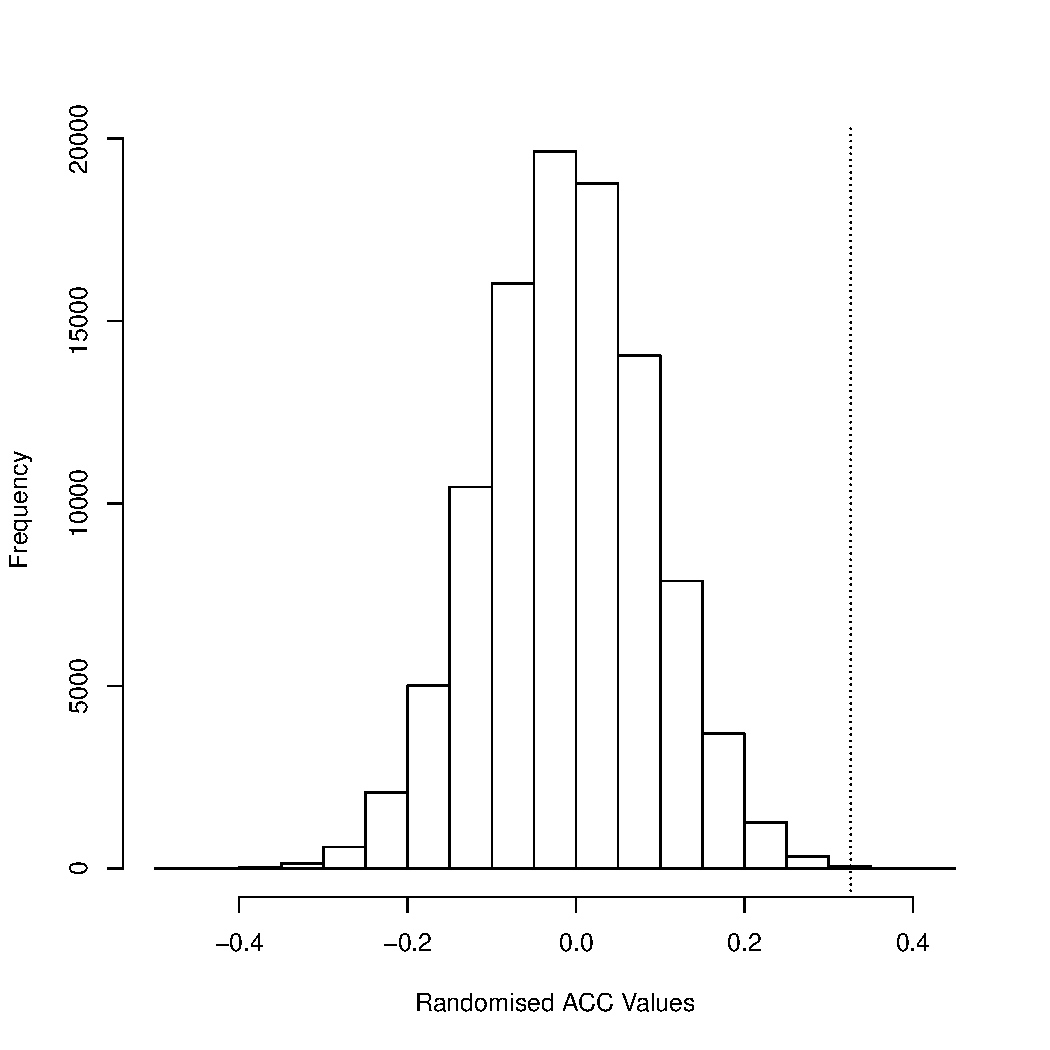
\includegraphics[width = 4in, height = 5in]{../data/ACC_Hist.pdf}
\caption{A histogram showing the distribution of autocorrelation 
coefficients from 10,000 randomly reordered versions of our original dataset. 
The vertical dotted line denotes where 0.326, the true autocorrelation
coefficient of the data, would lie on the distribution.} 
\label{fig:Figure 2}
\end{figure}

\vspace{10mm} 

Of the 10,000 ACC values based on shuffled data, only 18 were larger than 
the ACC of the real data, 0.326. This gives us an estimated p-value of less than 
0.01.

We can therefore reject the null hyothesis, and accept that the autocorrelation 
of temperature between successive years is significant. 


\end{document}